\section*{Supplementary Note 5: Annotator Guidelines} \label{appendix:annotator guidelines}
\rev{We build on the rare disease mention annotations from \cite{dong2023ontology_poor_annotations} in MIMIC-III, first filtering out clearly erroneous annotations as detailed in Table \ref{tab:Filtering_Details_ex}. Following filtering, a Ph.D. student reviewed each remaining entity from \cite{dong2023ontology_poor_annotations} under physician guidance, applying the review process outlined in Fig. \ref{fig:annotator_guidelines} to determine whether each mention directly or indirectly implies a rare disease. This produced our final curated annotation set.}

\rev{For the RDMA-assisted annotation run, the same Ph.D. student conducted a separate review pass over only the entities flagged by RDMA for human review, applying a binary correction, marking each as correct or incorrect. RDMA flags entities exhibiting disagreement across two independent mining passes and a final agent verification check, meaning the annotator is presented only with the subset of entities where automated agreement could not be established.}

\rev{\paragraph{Inter-Annotator Agreement.} We measure agreement between the human annotator and RDMA using Cohen's $\kappa$, which corrects observed agreement by chance agreement:}
\begin{equation}
    \rev{\kappa = \frac{p_o - p_e}{1 - p_e}}
\end{equation}
\rev{Given a $2 \times 2$ confusion matrix over $N = \text{TP} + \text{TN} + \text{FP} + \text{FN}$ binary judgments, observed agreement and chance agreement are computed as:}
\begin{align}
    \rev{p_o} &\rev{= \frac{\text{TP} + \text{TN}}{N}} \\
    \rev{p_e} &\rev{= p_{\text{human}} \cdot p_{\text{RDMA}} + (1 - p_{\text{human}}) \cdot (1 - p_{\text{RDMA}})}
\end{align}
\rev{where $p_{\text{human}} = (\text{TP} + \text{FN}) / N$ and $p_{\text{RDMA}} = (\text{TP} + \text{FP}) / N$ are the marginal rates of each rater labeling an entity as a rare disease mention. We report $\kappa$ under the Landis \& Koch interpretation bands, where $\kappa \in [0.41, 0.60]$ indicates moderate agreement and $\kappa \in [0.81, 1.00]$ indicates almost perfect agreement. Agreement between the human annotator and the unassisted prior annotations yielded $\kappa = 0.454$ (moderate), while agreement between the human annotator and RDMA-assisted annotations yielded $\kappa = 0.810$ (almost perfect), demonstrating a substantial improvement in annotation quality under the RDMA-assisted workflow.}

\begin{figure}[h!]
    \centering
    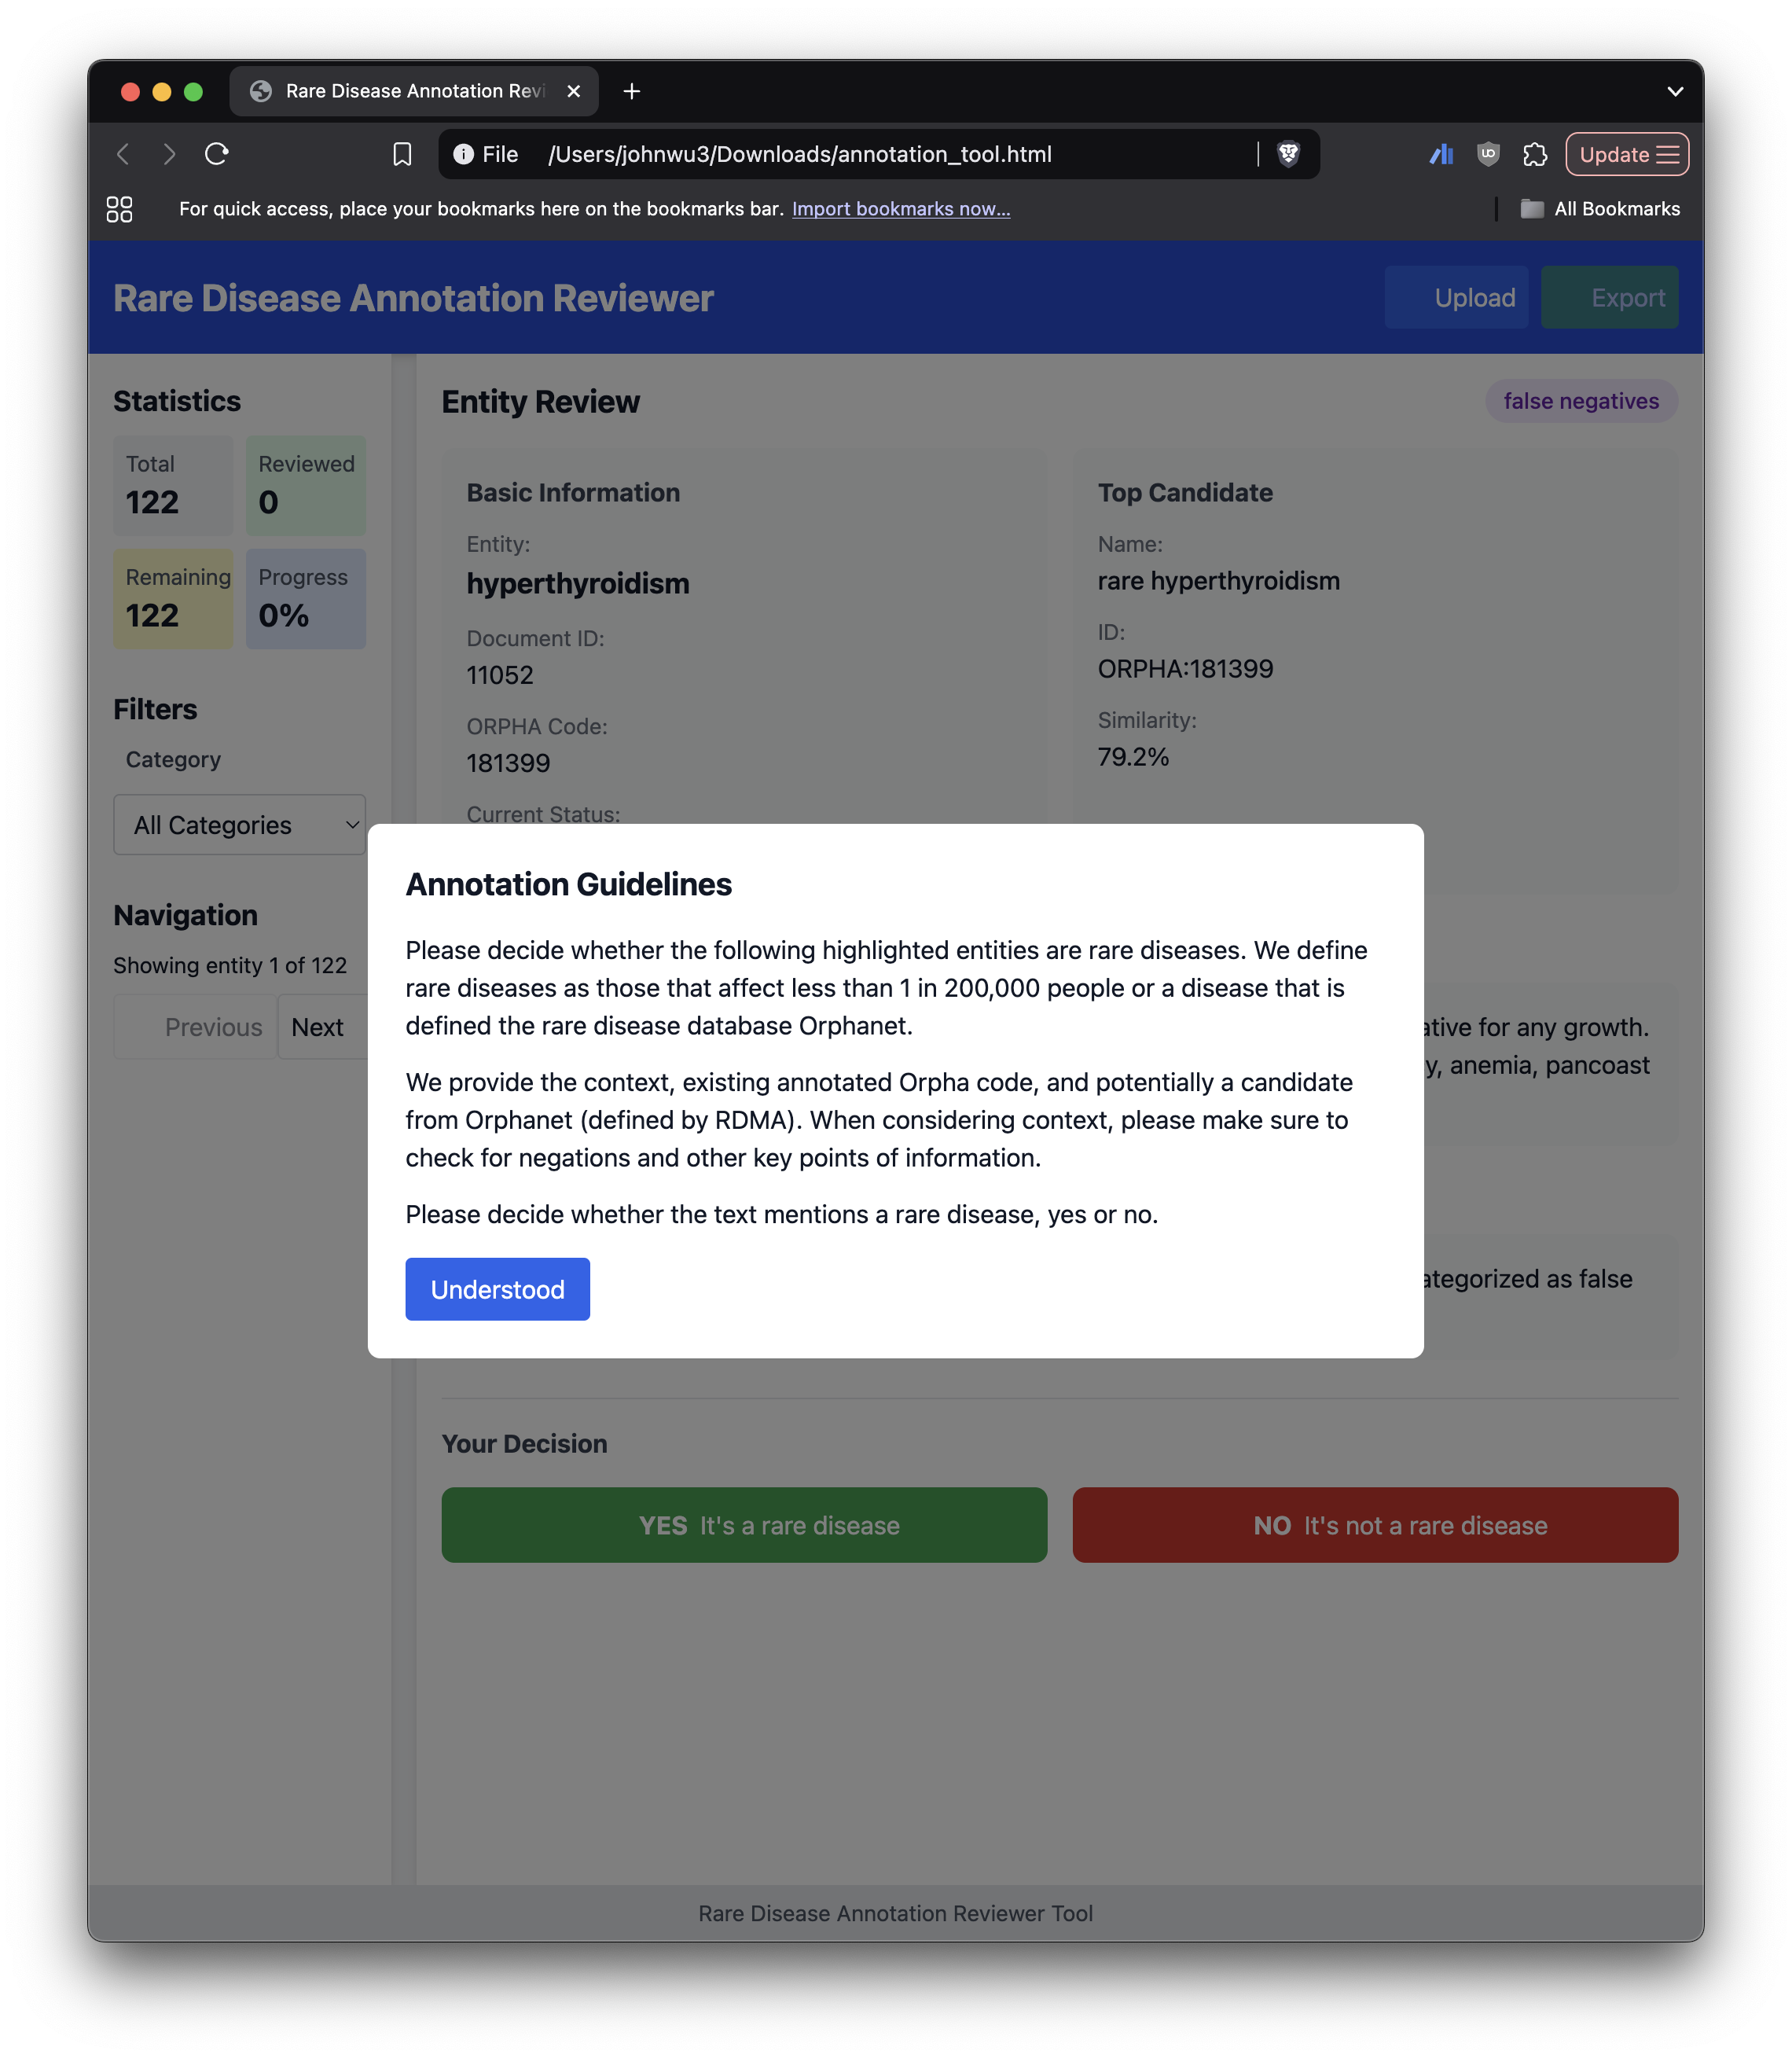
\includegraphics[width=0.8\textwidth]{figs/annotator_guidelines.png}
    \caption{\textbf{Annotator Guidelines.} Annotators are asked if the mention in text directly or indirectly implies a rare disease.}
    \label{fig:annotator_guidelines}
\end{figure}